\chapter{Related Works}

As we seen in the previous chapters, the quest for finding practically feasible reconstruction methods that need the least number of measurements (ideally close to the theoretical limits of the compressed sensing framework) is a challenging task; nonetheless, it is a hot topic having very important new results an novel approaches outperforming the older ones almost in every year. In this chapter we will discuss two recently published research projects both presenting a state-of-the-art solution, and we will review a third project that proposes an algorithm that has the potential to drastically outperform the methods currently considered to be the best on this field.

\section{Low Rank and Sparse Decomposition}

Initially the compressed sensing framework was implemented in classic sparsity seeking settings, and the main question was which transform domain has the sparsest representation of the signal of interest. Although the authors of the first compressed sensing publications were aware of the low rank structure of certain MRI techniques back in 2007, this branch of research gained larger attention just in the recent years. An approach that appeared to be particularly suitable to dynamic MRI setting is decomposition of the image into a low rank and a sparse component~\cite{lingala_accelerated_2011, tremoulheac_dynamic_2014, otazo_low-rank_2015, roohi_multi-dimensional_2017}. The motivation behind such a decomposition comes from the inherent temporal correlation of the background---that correlation is captured by the low rank part usually denoted by $L$---and from the sparse nature of dynamic information that lies on top of the background, encompassed by the sparse component with the notation of $S$.

A recent paper from Lin and Fessler~\cite{lin_efficient_2019}, published in 2019, attempts to summarize the advances in this field, then it proposes two new algorithms to accelerate the convergence of the most successful algorithms, and finally it presents the results of the numerical experiments they carried out to compare the convergence rate of different state-of-the-art algorithms.  

\subsubsection{Formulation of the Problem}
In contrast to the basic sparsity formulation discussed earlier as (\ref{eq:P_0}) problem and its relaxation to the (\ref{eq:P_1}) problem, the problem formulation of $L+S$ decomposition scheme (also called robust principal component analysis or RPCA) have two constraints in the place of the original constraint promoting sparsity in some transform domain. The first of these new constraints is the sparsity seeking $\ell_0$ norm that takes the sparse part as an argument, similarly to the original settings in (\ref{eq:P_0}). The other constraint, however, enforces the low-rankness of $L$. Putting it together, we get a LASSO-like formula
\[\min_{\mathbf{L,S}} \norm{\mathcal{A}\mathbf{(L+S) - y}}_F\; \text{ subject to }\; rank(\mathbf{L}) < r\; \text{ and }\; \norm{\Phi \mathbf{S}}_1 < s,\]
where $\mathcal{A}: \mathbb{C}^{N \times n_t} \rightarrow \mathbb{C}^{m \times n_c \times n_t}$ is a linear operator (often represented\footnote{This matrix representation requires the vectorization of the input before the matrix-vector multiplication; however, this operation is hardly ever indicated explicitly, but rather assumed to be performed implicitly. In this thesis work, we also omit denoting such vectorizations.} by a matrix in $\mathbb{C}^{m \cdot n_c \cdot n_t \times N \cdot n_t}$, especially in theoretical discussions) modelling the 2D parallel MRI acquisition scheme that assumes $N$ pixels in each frame, $n_c$ receiver coils and $n_t$ time frames that evaluates exactly $m$ k-space points. Moreover, $\Phi: \mathbb{C}^{N \times n_t} \rightarrow \mathbb{C}^{N \cdot n_t}$ is an appropriate sparsifying transform, $\mathbf{y}$ denotes the collection of measurement data, $\mathbf{L, S} \in \mathbb{C}^{N \times nt}$ hold the low rank and sparse components, and finally $r$ and $s$ are the target rank and sparsity. After solving this problem for $\mathbf{L}$ and $\mathbf{S}$, the reconstructed image can be obtained by the simple element-wise addition of components (of course, we need to reshape back the resulted matrix to be a 2D or 3D dynamic image instead $N\times n_t$ shape created by stacking the vectorized frames as the columns).

The most common scenario to solve the $L+S$ problem follows the same line of arguments that was presented earlier: Instead of solving the problem that contains an $\ell_0$ and a $rank$ term, both being NP-hard to optimize even separately, one can relax both constraints to $\ell_1$-norm and nuclear norm minimization, respectively, resulting the Lagrangian formula
\[\min_{\mathbf{L,S}} \norm{\mathcal{A}\mathbf{(L+S) - y}}_2 + \lambda_L \norm{\mathbf{L}}_* + \lambda_S \norm{\Phi \mathbf{S}}_1.\]

In the aforementioned paper, the authors considered the unitary temporal Fourier transform $\mathbb{T}_t$ as the sparsifying operator $\Phi$, which is a largely conventional for dynamic MR images, and they divided the analyzed algorithms into two main groups: methods based on proximal gradient technique and algorithms using variable splitting then solving the transformed problem in the augmented Lagrangian framework, possibly using the ADMM scheme.

\subsubsection{Proximal Gradient Methods}
In the first group they studied the three shrinkage-thresholding algorithms: ISTA, FISTA and POGM. While ISTA has already been utilized along with the $L+S$ modelling scheme in~\cite{otazo_low-rank_2015}, it was their contribution to show the applicability of accelerated schemes in this setting. First, they combined $\mathbf{L}$ and $\mathbf{S}$ into a single "stacked" variable $\mathbf{X} = \left[\begin{matrix}\mathbf{L} & \mathbf{S}\end{matrix}\right]^T$ to simplify the notation because that way the momentum step can be expressed by a single equation. Second, they recalled that the proximity operator has closed formula; namely, the composition soft-thresholding function with the sparsity transform and the singular-value thresholding, the latter defined as
\[SVT_{\lambda_L}(\mathbf{L}) = \mathbf{U}\Lambda_\lambda(\boldsymbol{\Sigma})\mathbf{V}*,\]
first proposed to enforce low-rankness in~\cite{cai_singular_2008}. Note that $\mathbf{U}\boldsymbol{\Sigma}\mathbf{V}*$ in the formula above stands for the singular value decomposition of the input matrix $\mathbf{L}$. Consequently, the forward-backward splitting scheme is easily applied to both variable performing
\begin{align*}
    & \mathbf{L}_k = SVT_{\lambda_L}(\mathbf{L}_{k-1} - t \nabla_L g(\mathbf{X}_{k-1})\\
    & \mathbf{S}_k = \mathbf{T}*\left(\Lambda_{\lambda_S}\left(\mathbf{T}(\mathbf{S}_{k-1} - t \nabla_S g(\mathbf{X}_{k-1})\right)\right),
\end{align*}
where $g(\mathbf{X}) = \frac{1}{2}\norm{[\mathcal{A} \; \mathcal{A}]\mathbf{X} - \mathbf{y}}_2^2$ and therefore \[\nabla_L\; g(\mathbf{X}) = \nabla_S\; g(\mathbf{X}) = \mathcal{A}^*([\mathcal{A} \; \mathcal{A}]\mathbf{X} - \mathbf{y}) = \mathcal{A}^*(\mathcal{A} (\mathbf{L + S}) - \mathbf{y}).\] Accordingly, the algorithm takes form presented in algorithm~\ref{alg:ista-LS}.

\begin{algorithm}
    \SetKwInOut{Input}{input}
    \SetKwInOut{Output}{output}
    \Input{
        $\mathbf{y}$: undersampled k-space data\\
        $\mathcal{A}$: data acquisition operator\\
        $\mathbf{T}$: temporal Fourier transform\\
        $\lambda_L$: singular value threshold\\
        $\lambda_S$: sparsity threshold\\
        $N$: number of iterations}
    \Output{$\mathbf{L, S} = \argmin_{\mathbf{L, S}}  \norm{\mathcal{A}\mathbf{(L+S) - y}}_2 + \lambda_L \norm{\mathbf{L}}_* + \lambda_S \norm{\mathbf{T} \mathbf{S}}_1$}
    \BlankLine
    initialization: $\mathbf{L}_0 = \mathcal{A}^* \mathbf{d}, \mathbf{S}_0 = \mathbf{0}, \theta_0 = 1, t = 0.99$\\
    notation: $\mathbf{X}_i = \begin{bmatrix}\mathbf{L}_i \\ \mathbf{S}_i\end{bmatrix}$\\
    \For{$k = 1 \ldots N$}{
        $\nabla g_k = \mathcal{A}^*(\mathcal{A} (\mathbf{L_{k-1} + S_{k-1}}) - \mathbf{y})$\\
        $\mathbf{L}_k = SVT_{\lambda_L}(\mathbf{L}_{k-1} - t \nabla g_k)$\\
        $\mathbf{S}_k = \mathbf{T}^*\left(\Lambda_{\lambda_S}\left(\mathbf{T}(\mathbf{S}_{k-1} - t \nabla g_k)\right)\right)$
    }
    \Return{$\mathbf{L}_N + \mathbf{S}_N$}
    \caption{ISTA for L+S decomposition}
    \label{alg:ista-LS}
\end{algorithm}

\begin{algorithm}
    \SetKwInOut{Input}{input}
    \SetKwInOut{Output}{output}
    \Input{same as input of algorithm~\ref{alg:ista-LS}}
    \Output{$\mathbf{L, S} = \argmin_{\mathbf{L, S}}  \norm{\mathcal{A}\mathbf{(L+S) - y}}_2 + \lambda_L \norm{\mathbf{L}}_* + \lambda_S \norm{\mathbf{T} \mathbf{S}}_1$}
    \BlankLine
    initialization: $\mathbf{L}_0 = \mathcal{A}^* \mathbf{d}, \mathbf{S}_0 = \mathbf{0}, \theta_0 = 1, t = 0.5$\\
    notation: $\mathbf{X}_i = \begin{bmatrix}\mathbf{L}_i \\ \mathbf{S}_i\end{bmatrix}, \mathbf{\tilde{X}}_i = \begin{bmatrix}\mathbf{\tilde{L}}_i \\ \mathbf{\tilde{S}}_i\end{bmatrix}, \mathbf{\bar{X}}_i = \begin{bmatrix}\mathbf{\bar{L}}_i \\ \mathbf{\bar{S}}_i\end{bmatrix}$\\
    \For{$k = 1 \ldots N$}{
        $\nabla g_k = \mathcal{A}^*(\mathcal{A} (\mathbf{L_{k-1} + S_{k-1}}) - \mathbf{y})$\\
        
        $\mathbf{\tilde{L}}_k = \mathbf{L}_{k-1} - t \nabla g_k$\\
        $\mathbf{\tilde{S}}_k = \mathbf{S}_{k-1} - t \nabla g_k$\\
        
        $\theta_k = \frac{1}{2}\left(1 + \sqrt{1 + 4\theta_{k-1}^2}\right)$\\
        
        $\mathbf{\mathbf{\bar{X}}}_k = \mathbf{\tilde{X}}_k + \frac{\theta_{k-1}-1}{\theta_k}(\tilde{X}_k - \mathbf{\tilde{X}}_{k-1}) + \frac{\theta_{k-1}}{\theta_k}(\mathbf{\tilde{X}}_k - \mathbf{X}_{k-1})$\\
        
        $\mathbf{L}_k = SVT_{\lambda_L}(\mathbf{\bar{L}}_k)$\\
        $\mathbf{S}_k = \mathbf{T}^*\left(\Lambda_{\lambda_S}\left(\mathbf{T}(\mathbf{\bar{L}}_k)\right)\right)$
    }
    \Return{$\mathbf{L}_N + \mathbf{S}_N$}
    \caption{FISTA for L+S decomposition}
    \label{alg:fista-LS}
\end{algorithm}

\begin{algorithm}[tb]
    \SetKwInOut{Input}{input}
    \SetKwInOut{Output}{output}
    \Input{same as input of algorithm~\ref{alg:ista-LS}}
    \Output{$\mathbf{L, S} = \argmin_{\mathbf{L, S}}  \norm{\mathcal{A}\mathbf{(L+S) - y}}_2 + \lambda_L \norm{\mathbf{L}}_* + \lambda_S \norm{\mathbf{T} \mathbf{S}}_1$}
    \BlankLine
    initialization: $\mathbf{L}_0 = \mathcal{A}^* \mathbf{d}, \mathbf{S}_0 = \mathbf{0}, \theta_0 = \zeta_0 = 1, t = 0.5$\\
    notation: $\mathbf{X}_i = \begin{bmatrix}\mathbf{L}_i \\ \mathbf{S}_i\end{bmatrix}, \mathbf{\tilde{X}}_i = \begin{bmatrix}\mathbf{\tilde{L}}_i \\ \mathbf{\tilde{S}}_i\end{bmatrix}, \mathbf{\bar{X}}_i = \begin{bmatrix}\mathbf{\bar{L}}_i \\ \mathbf{\bar{S}}_i\end{bmatrix}$\\
    \For{$k = 1 \ldots N$}{
        $\nabla g_k = \mathcal{A}^*(\mathcal{A} (\mathbf{L_{k-1} + S_{k-1}}) - \mathbf{y})$\\
        
        $\mathbf{\tilde{L}}_k = \mathbf{L}_{k-1} - t \nabla g_k$\\
        $\mathbf{\tilde{S}}_k = \mathbf{S}_{k-1} - t \nabla g_k$\\
        
        $\theta_k = \begin{cases} \frac{1}{2}\left(1+\sqrt{1 + 4\theta_{k-1}^2}\right) : k < N \\ \frac{1}{2}\left(1+\sqrt{1 + 8\theta_{k-1}^2}\right) : k = N \end{cases}$\\
        
        $\mathbf{\mathbf{\bar{X}}}_k = \mathbf{\tilde{X}}_k + \frac{\theta_{k-1}-1}{\theta_k}(\tilde{X}_k - \mathbf{\tilde{X}}_{k-1}) + \frac{\theta_{k-1}}{\theta_k}(\mathbf{\tilde{X}}_k - \mathbf{X}_{k-1}) + \frac{\theta_{k-1}-1}{\zeta_{k-1} \theta_k}(\mathbf{\bar{X}}_{k-1} - \mathbf{X}_{k-1})$\\
        
        $\zeta_k = t(1+\frac{\theta_{k-1}-1}{\theta_k} + \frac{\theta_{k-1}}{\theta_k})$
        
        $\mathbf{L}_k = SVT_{\lambda_L}(\mathbf{\bar{L}}_k)$\\
        $\mathbf{S}_k = \mathbf{T}^*\left(\Lambda_{\lambda_S}\left(\mathbf{T}(\mathbf{\bar{L}}_k)\right)\right)$
    }
    \Return{$\mathbf{L}_N + \mathbf{S}_N$}
    \caption{POGM for L+S decomposition}
    \label{alg:pogm-LS}
\end{algorithm}


Next, they extended this base algorithm to the accelerated scheme by inserting a momentum step that resulted in algorithm~\ref{alg:fista-LS} for FISTA and algorithm~\ref{alg:pogm-LS} for POGM. For the sake of clarity and completeness, we note that the authors used a slightly different formulation than the algorithms presented here, as they followed the original formulation of ISTA given in~\cite{otazo_low-rank_2015}. The main difference is that they calculated the gradient at the \textit{end} of the loop body, not in the beginning, and they introduced an additional variable $\mathbf{M}$, named \textit{consistency term}, that was defined as 
\[\mathbf{M = L + S - \mathbf{E}^*(\mathbf{E} (\mathbf{L_{k-1} + S_{k-1}}) - \mathbf{d})}\] ($\mathbf{E}$ and $\mathbf{d}$ corresponds to $\mathcal{A}$ and $\mathbf{y}$ in our notation). While this version avoids an unnecessary calculation of gradient in the very first iteration, it introduces a couple avoidable matrix additions in turn, and also it makes more difficult to understand how the algorithms are connected to the original, only sparsity seeking versions. We summarized all three algorithms in algorithm~\ref{alg:lin_pgm}, following their notation, and it is easy to see that there is no significant difference between the two formulations, but our version is easier to understand.

\begin{algorithm}
    \SetKwInOut{Input}{input}
    \SetKwInOut{Output}{output}
    \Input{same as input of algorithm~\ref{alg:ista-LS}}
    \Output{$\mathbf{L, S} = \argmin_{\mathbf{L, S}}  \norm{\mathcal{A}\mathbf{(L+S) - y}}_2 + \lambda_L \norm{\mathbf{L}}_* + \lambda_S \norm{\mathbf{T} \mathbf{S}}_1$}
    \BlankLine
    initialization: $\mathbf{M}_0 = \mathbf{L}_0 = \mathcal{A}^* \mathbf{d}, \mathbf{S}_0 = \mathbf{0}, \theta_0 = \zeta_0 = 1, t = \begin{cases}1 : \text{ISTA} \\ 0.5 : \text{FISTA and POGM}\end{cases}$\\
    notation: $\mathbf{X}_i = \begin{bmatrix}\mathbf{L}_i \\ \mathbf{S}_i\end{bmatrix}, \mathbf{\tilde{X}}_i = \begin{bmatrix}\mathbf{\tilde{L}}_i \\ \mathbf{\tilde{S}}_i\end{bmatrix}, \mathbf{\bar{X}}_i = \begin{bmatrix}\mathbf{\bar{L}}_i \\ \mathbf{\bar{S}}_i\end{bmatrix}$\\
    \For{$k = 1 \ldots N$}{
        
        $\mathbf{\tilde{L}}_k = \mathbf{M}_{k-1} - \mathbf{L}_{k-1}$\\
        $\mathbf{\tilde{S}}_k = \mathbf{M}_{k-1} - \mathbf{S}_{k-1}$\\
        
        \uIf{ISTA}{
            $\mathbf{\mathbf{\bar{X}}}_k = \mathbf{\tilde{X}}$
        }
        \uElseIf{FISTA}{
            $\theta_k = \frac{1}{2}\left(1+\sqrt{1 + 4\theta_{k-1}^2}\right)$\\
            $\mathbf{\mathbf{\bar{X}}}_k =
            \mathbf{\tilde{X}}_k + \frac{\theta_{k-1}-1}{\theta_k}(\tilde{X}_k - \mathbf{\tilde{X}}_{k-1}) + \frac{\theta_{k-1}}{\theta_k}(\mathbf{\tilde{X}}_k - \mathbf{X}_{k-1})$\\
        }
        \ElseIf{POGM}{
            $\theta_k = \begin{cases} \frac{1}{2}\left(1+\sqrt{1 + 4\theta_{k-1}^2}\right) : k < N \\ \frac{1}{2}\left(1+\sqrt{1 + 8\theta_{k-1}^2}\right) : k = N \end{cases}$\\
            $\mathbf{\mathbf{\bar{X}}}_k =
            \mathbf{\tilde{X}}_k + \frac{\theta_{k-1}-1}{\theta_k}(\tilde{X}_k - \mathbf{\tilde{X}}_{k-1}) + \frac{\theta_{k-1}}{\theta_k}(\mathbf{\tilde{X}}_k - \mathbf{X}_{k-1}) + \frac{\theta_{k-1}-1}{\zeta_{k-1} \theta_k}(\mathbf{\bar{X}}_{k-1} - \mathbf{X}_{k-1})$\\
            $\zeta_k = t(1+\frac{\theta_{k-1}-1}{\theta_k} + \frac{\theta_{k-1}}{\theta_k})$
        }
        
        $\mathbf{L}_k = SVT_{\lambda_L}(\mathbf{\bar{L}}_k)$\\
        $\mathbf{S}_k = \mathbf{T}^*\left(\Lambda_{\lambda_S}\left(\mathbf{T}(\mathbf{\bar{L}}_k)\right)\right)$\\
        
        $\mathbf{M}_k = \mathbf{L}_k + \mathbf{S}_k - \mathcal{A}^*(\mathcal{A} (\mathbf{L_k + S_k}) - \mathbf{y})$
    }
    \Return{$\mathbf{L}_N + \mathbf{S}_N$}
    \caption{ISTA/FISTA/POGM for L+S, as formulated in~\cite{lin_efficient_2019}}
    \label{alg:lin_pgm}
\end{algorithm}

\subsubsection{Augmented Lagrangian Methods}
The other approach they studied based on the augmented Lagrangian formulation combined with the variable splitting scheme. The conventional way, proposed in~\cite{tremoulheac_dynamic_2014}, to perform the variable splitting transform the original $L+S$ problem into 
\[\min_{\mathbf{L,S}}\min_{\mathbf{P,Q}} \left\{\frac{1}{2}\norm{\mathcal{A}(\mathbf{L+S}) - \mathbf{y}}_2^2 + \lambda_L \norm{\mathbf{P}}_* + \lambda_S \norm{\mathbf{Q}}_1\right\} \textrm{ subject to } \begin{cases} \mathbf{P = L} \\ \mathbf{Q = TS} \end{cases}.\]
Using ADMM technique, this formulation yields a modified augmented Lagrangian function
\begin{align*}
L(\mathbf{L, S, P, Q, V}_1, \mathbf{V}_2) = & \frac{1}{2}\norm{\mathcal{A}(\mathbf{L+S}) - \mathbf{y}}_2^2 + \lambda_L \norm{\mathbf{P}}_* + \lambda_S \norm{\mathbf{Q}}_1 + \ldots \\ & + \frac{\delta_1}{2}\norm{\mathbf{L - P + V}_1}_2^2 + \frac{\delta_2}{2}\norm{\mathbf{TS - Q + V}_2}_2^2,
\end{align*}
where $\mathbf{V}_1$ and $\mathbf{V}_2$ take the place of Lagrangian multipliers in the classic augmented Lagrangian method, and they come from the relaxation of equality constraints $\mathbf{P = L}$ and $\mathbf{Q = TS}$ to $\mathbf{L - P = V}_1$ and $\mathbf{TS - Q = V}_2$. Thus, setting $\mathbf{V}_1$ and $\mathbf{V}_2$ to $\mathbf{0}$ leads back to the solution of the constrained problem. These variables are adjusted after each step to penalize deviations from the equality constraints, specifically for each pixel.

The associated algorithm (algorithm~\ref{alg:al-cg}) consists of four main steps, each optimizing $L$ function for one variable while fixing all others. The minimization for $\mathbf{P}$ and $\mathbf{Q}$ is quite straightforward as they can solved by the proximity operators: the soft-thresholding solves for the $\ell_1$-norm constraint on $\mathbf{Q}$ and $SVT$ minimizes for the nuclear norm. Although these steps also needs to take care of the other two terms introduced by the equality constraints, they still have a directly solvable formula. On the other hand, optimization for $\mathbf{L}$ and $\mathbf{S}$ needs more elaborate steps. In fact, the most general solution is utilized by the authors of the paper; namely, they try to find the root of the gradient. As all terms containing $\mathbf{L}$ and $\mathbf{S}$ are $\ell_2$ norms, the best (first-order) iterative method to find the root of these quadratic terms is certainly the conjugate gradient. The inputs of CG are derived as follows. Let us first take the partial derivate of the augmented Lagrangian:
\[\frac{\partial}{\partial L} L(\mathbf{L, S, P, Q, V}_1, \mathbf{V}_2) = \mathcal{A}^*(\mathcal{A}(\mathbf{L} + \mathbf{S}) - \mathbf{y}) + \delta_1(\mathbf{L + P - V}_1) \overset{!}{=} \mathbf{0}.\]
Then we can separate $\mathbf{L}$ from the rest of the formula by rearranging
\begin{align*}
    \mathcal{A}^*(\mathcal{A}(\mathbf{L} + &\mathbf{S}) - \mathbf{y}) + \delta_1(\mathbf{L + P - V}_1) = \mathcal{A}^*\mathcal{A}\mathbf{L} + \mathcal{A}^*\mathcal{A}\mathbf{S} - \mathcal{A}^*\mathbf{y} + \delta_1\mathbf{L} + \delta_1(\mathbf{P - V}_1) = \ldots \\ & = (\mathcal{A}^*\mathcal{A} + \delta_1\mathbf{I})\mathbf{L} + \mathcal{A}^*\mathcal{A}\mathbf{S} - \mathcal{A}^*\mathbf{y} + \delta_1(\mathbf{P - V}_1).
\end{align*}
Finally, putting it back to the previous equation and performing some further rearrangements, we get the equation
\[(\mathcal{A}^*\mathcal{A} + \delta_1\mathbf{I})\mathbf{L} = \mathcal{A}^*\mathcal{A}\mathbf{S} - \mathcal{A}^*\mathbf{y} + \delta_1\mathbf{P - V}_1\]
that fits the CG scheme as $\mathcal{A}^*\mathcal{A} + \delta_1\mathbf{I}$ is Hermitian and positive definite. Following the same line of arguments, the equation needs to be minimized for $\mathbf{S}$ is derived as 
\[(\mathcal{A}^*\mathcal{A} + \delta_2\mathbf{I})\mathbf{S} = \mathcal{A}^*\mathcal{A}\mathbf{L} - \mathcal{A}^*\mathbf{y} + \delta_1\mathbf{Q - V}_2.\]

\begin{algorithm}[tb]
    \SetKwInOut{Input}{input}
    \SetKwInOut{Output}{output}
    \Input{
        $\mathbf{y}$: undersampled k-space data\\
        $\mathcal{A}$: data acquisition operator\\
        $\mathbf{T}$: temporal Fourier transform\\
        $\lambda_L$: singular value threshold\\
        $\lambda_S$: sparsity threshold\\
        $maxIter_L$: number of conjugate gradient iteration steps for $L$\\
        $maxIter_S$: number of conjugate gradient iteration steps for $S$\\
        $\delta_1$, $\delta_2$: AL penalty parameters\\
        $N$: number of iterations}
    \Output{$\mathbf{L, S} = \argmin_{\mathbf{L, S}}  \norm{\mathcal{A}\mathbf{(L+S) - y}}_2 + \lambda_L \norm{\mathbf{L}}_* + \lambda_S \norm{\mathbf{T} \mathbf{S}}_1$}
    \BlankLine
    initialization: $\mathbf{L}_0 = \mathcal{A}^* \mathbf{y}, \mathbf{S}_0 = \mathbf{V}_{1,0} = \mathbf{V}_{2,0} = \mathbf{0}$\\
    \For{$k = 1 \ldots N$}{
        $\mathbf{P}_k = SVT_{\lambda_L / \delta_1} (\mathbf{L}+\mathbf{V}_{2,k})$\\
        $\mathbf{Q}_k = \mathbf{T}^* \Lambda_{\lambda_S / \delta_2} (\mathbf{T}S) + \mathbf{V}_{2,k} $\\
        $\mathbf{L}_k = \argmin_{\mathbf{L}} (\mathcal{A}^*\mathcal{A} + \delta_1\mathbf{I})\mathbf{L} = \mathcal{A}^*\mathbf{y} - \mathcal{A}^*\mathcal{A}\mathbf{S} + \delta_1(\mathbf{P} - \mathbf{V}_{1,k}) \text{ starting from }\mathbf{L}_{k-1}$\\
        $\mathbf{S}_k = \argmin_{\mathbf{S}} (\mathcal{A}^*\mathcal{A} + \delta_2\mathbf{I})\mathbf{S} = \mathcal{A}^*\mathbf{y} - \mathcal{A}^*\mathcal{A}\mathbf{S} + \delta_2(\mathbf{Q} - \mathbf{V}_{2,k}) \text{ starting from }\mathbf{S}_{k-1}$\\
        $\mathbf{V}_{1,k} = \mathbf{V}_{1,k-1} + \mathbf{L}_k - \mathbf{P}$\\
        $\mathbf{V}_{2,k} = \mathbf{V}_{2,k-1} + \mathbf{T}\mathbf{S}_k - \mathbf{Q}$
    }
    \Return{$\mathbf{L}_N + \mathbf{S}_N$}
    \caption{AL method with CG steps}
    \label{alg:al-cg}
\end{algorithm}

The second AL-type method that Lin and Fessler considered in their paper is a new method that decomposes the acquisition operator $\mathcal{A}$ into a coil sensitivity mapping $\mathcal{C}:\mathbb{C}^{N \times n_t} \rightarrow \mathbb{C}^{N \times n_c \times n_t}$ (briefly discussed in section~\ref{section:accelerated}), a spacial Fourier transform operator $\mathcal{F}: \mathbb{C}^{N \times n_c \times n_t} \rightarrow \mathbb{C}^{N \times n_c \times n_t}$, and an undersampling masking $\Omega: \mathbb{C}^{N \times n_c \times n_t} \rightarrow \mathbb{C}^{m \times n_c \times n_t}$ such that $\mathcal{A} = \Omega\mathcal{FC}$. They also assumed that $\mathcal{C}$ normalized and therefore it is also unitary; i.e., $\mathcal{C}^*\mathcal{C} = \mathbf{I}$. They can assume it without loss of generality as the image can be freely scaled without changing its rank or sparsity, and this is also true for the temporal Fourier domain. At the construction of the algorithm, they took advantage of the increased freedom in the choice of variable splitting. In particular, they split the acquisition operator together with the variables, and they arrived to the objective
\[\argmin_{\mathbf{L,S}}\min_{\mathbf{Z,X}}\left\{\frac{1}{2}\norm{\Omega \mathbf{Z -d}}_2^2 + \lambda_L \norm{\mathbf{L}}_* + \lambda_S \norm{\mathbf{TS}}_1\right\} \text{ subject to } \begin{cases} \mathbf{Z} = \mathcal{FC}\mathbf{X} \\ \mathbf{X = L + S} \end{cases}.\]
Afterwards, they defined the AL function by
\begin{align*}
    \argmin_{\mathbf{L,S}}&\min_{\mathbf{Z,X}}\left\{\frac{1}{2}\norm{\Omega \mathbf{Z -d}}_2^2 + \lambda_L \norm{\mathbf{L}}_* + \lambda_S \norm{\mathbf{TS}}_1\right\}\\
    & + \frac{\delta_1}{2}\norm{\mathcal{FC}\mathbf{X - Z + V}_1}_2^2 + \frac{\delta_2}{2}\norm{\mathbf{L + S - X + V}_2}_2^2,
\end{align*}
and they solved the resulting steps, as follows, exploiting that both $\mathbf{T}$ and $\mathcal{F}$ is unitary, introducing an auxiliary variable $\mathbf{\tilde{S}} = \mathbf{TS}$, and using again soft-thresholding and singular-value thresholding for $\ell_1$ and nuclear norm minimization:
\begin{itemize}[label={}]
    \item $\begin{aligned}
        \mathbf{Z}_k
        & = \argmin_\mathbf{Z} \frac{1}{2} \norm{\Omega \mathbf{Z - y}}_2^2 + \frac{\delta_1}{2}\norm{\mathbf{X - (L + S) + V}_2}_2^2\\
        & = \left(\Omega^*\Omega + \delta_1 \mathbf{I})^{-1}(\Omega^*\mathbf{y} + \delta_1(\mathcal{FC}\mathbf{X - V}_1)\right)
    \end{aligned}$
    \item $\begin{aligned}
        \mathbf{X}_k
        & = \argmin_\mathbf{X} \left\{ \frac{\delta_1}{2} \norm{\mathbf{Z} - \mathcal{FC}\mathbf{X + V}_1}_2^2 + \frac{\delta_2}{2} \norm{\mathbf{X - (L + S) + V}_2}_2^2 \right\}\\
        & = \left(\mathcal{C}^*\mathcal{C} + \frac{\delta_1}{\delta_2}\mathbf{I}\right)^{-1}\left(\mathcal{C}^*\mathcal{F}^* (\mathbf{Z + V}_1) + \frac{\delta_1}{\delta_2}(\mathbf{L+S+V}_2)\right)\\
        & = \frac{\delta_1}{\delta_1+\delta_2}\left(\mathcal{C}^*\mathcal{F}^* (\mathbf{Z+V}_1) + \frac{\delta_2}{\delta_1}(\mathbf{L+S-V}_2)\right)
    \end{aligned}$
    \item $\begin{aligned}
        \mathbf{L}_k
        & = \argmin_\mathbf{L} \left\{ (\lambda_L \norm{\mathbf{L}}_* + \frac{\delta_2}{2} \norm{\mathbf{X - (L + S) + V}_2}_2^2) \right\}\\
        & = SVT_{\lambda_L / \delta_2} (\mathbf{X-S+V}_2)
    \end{aligned}$
    \item $\begin{aligned}
        \mathbf{S}_k
        & = \argmin_\mathbf{S} \left\{ (\lambda_S \norm{\mathbf{TS}}_1 + \frac{\delta_2}{2} \norm{\mathbf{X - (L + S) + V}_2}^2) \right\}\\
        & = \mathbf{T}^* \left(\argmin_\mathbf{\tilde{S}} \left\{\lambda_S \norm{\mathbf{\mathbf{\tilde{S}}}}_1 + \frac{\delta_2}{2} \norm{\mathbf{T(X - (L + S) + V}_2) - \mathbf{\mathbf{\tilde{S}}}}_2^2\right\}\right)\\
        & = \mathbf{T}^* \Lambda_{\lambda_S / \delta_2} (\mathbf{T}(\mathbf{X - L + V}_2)).
    \end{aligned}$
\end{itemize}
Although these steps might look more complicated at first than the previous method, they can be calculated much faster indeed. In fact, the only inverse that needs to be calculated is $(\Omega^*\Omega + \delta_1 \mathbf{I})^{-1}$, but this calculation is quite cheap because $\Omega^*\Omega$ is diagonal. Algorithm~\ref{alg:al-2} summarizes the implementation of these steps, and describes the updates of the Lagrange multipliers.

\begin{algorithm}[tb]
    \SetKwInOut{Input}{input}
    \SetKwInOut{Output}{output}
    \Input{
        $\mathbf{y}$: undersampled k-space data\\
        $\mathcal{C}$: coil sensitivity operator\\
        $\mathcal{F}$: spacial Fourier transform operator\\
        $\Omega$: undersampling masking\\
        $\mathbf{T}$: temporal Fourier transform\\
        $\lambda_L$: singular value threshold\\
        $\lambda_S$: sparsity threshold\\
        $\delta_1$, $\delta_2$: AL penalty parameters\\
        $N$: number of iterations}
    \Output{$\mathbf{L, S} = \argmin_{\mathbf{L, S}}  \norm{\mathcal{A}\mathbf{(L+S) - y}}_2 + \lambda_L \norm{\mathbf{L}}_* + \lambda_S \norm{\mathbf{T} \mathbf{S}}_1$}
    \BlankLine
    initialization: $\mathbf{X}_0 = \mathbf{L}_0 = \mathcal{C}^*\mathcal{F}^*\Omega^* \mathbf{y}, \mathbf{S}_0 = \mathbf{V}_{1,0} = \mathbf{V}_{2,0} = \mathbf{0}$\\
    \For{$k = 1 \ldots N$}{
        $\mathbf{Z}_k = \left(\Omega^*\Omega + \delta_1 \mathbf{I})^{-1}(\Omega^*\mathbf{y} + \delta_1(\mathcal{FC}\mathbf{X - V}_1)\right)$\\
        $\mathbf{X}_k = \frac{\delta_1}{\delta_1+\delta_2}\left(\mathcal{C}^*\mathcal{F}^* (\mathbf{Z+V}_1) + \frac{\delta_2}{\delta_1}(\mathbf{L+S-V}_2)\right)$\\
        $\mathbf{L}_k = SVT_{\lambda_L / \delta_2} (\mathbf{X-S+V}_2)$\\
        $\mathbf{S}_k = \mathbf{T}^* \Lambda_{\lambda_S / \delta_2} (\mathbf{T}(\mathbf{X - L + V}_2))$\\
        $\mathbf{V}_{1,k} = \mathbf{V}_{1,k-1} + (\mathbf{Z}_k - \mathcal{FC}\mathbf{X}_k)$\\
        $\mathbf{V}_{2,k} = \mathbf{V}_{2,k-1} + \mathbf{X}_k - (\mathbf{L}_k + \mathbf{S}_k)$
    }
    \Return{$\mathbf{L}_N + \mathbf{S}_N$}
    \caption{improved AL method}
    \label{alg:al-2}
\end{algorithm}

\subsubsection{Datasets and Results}
To evaluate the convergence speed and time complexity of the examined algorithms, they performed numerical experiments on three Cartesian datasets and one another recorded via a non-Cartesian sampling trajectory. Two of the Cartesian images and the non-Cartesian one were published as a supplement to~\cite{otazo_low-rank_2015}, and a simulated Cartesian dataset is taken from~\cite{nakarmi_accelerating_2016}---which, in turn, was generated by the MRXCAT toolbox~\cite{wissmann_mrxcat_2014} that aims to provide realistic numerical phantoms for cardiovascular magnetic resonance. Their results on all datasets were consistent proving the claimed improvement induced by the two methods they proposed. They found that POGM outperforms all other methods in case of all the four datasets, the "second place" is shared between FISTA and the improved AL scheme, and the AL method with CG inner steps appears to be the slowest in both convergence rate and time complexity. The latter is mainly due to the time consuming CG steps, but also the improved AL algorithm is computationally more expensive. This comparison, however, is slightly unfair since it fails to consider a very important advantage of ADMM-like methods, notably the independence of steps that allows highly parallel implementations. Nonetheless, the primacy of POGM---which, in fact, is the most important result of the research project---is inevitable.

\subsection{Multiscale Low Rank Decomposition}

A similarly outstanding result was published by Frank Ong in the form of a doctoral dissertation~\cite{ong_low_2018} in 2018, and as a preprint of a journal paper~\cite{ong_extreme_2020} submitted in December, 2019 (accepted in April, 2020~\cite{ong_extreme_2020-1}). The novelty of his approach is that he makes the so called \textit{multiscale low rank} (MSLR) scheme practically feasible and demonstrates its effectiveness in MRI setting. The idea was first proposed by McCoy et al.~\cite{mccoy_achievable_2013, mccoy_convexity_2014, mccoy_sharp_2014}, and it naturally extended the $L+S$ scheme by filling the "gap" between the large scale low rankness, which is a global property, and pixel level sparsity, both being unable to capture the local structures. Dynamic MR images of the full body, for instance, exhibits large scale motions such as respiratory motion or change in body posture. On the other hand, heart beats and motions of the gastrointestinal tract are better described in a smaller scale, and movements of veins have effect on an even smaller scale.

The MSLR approach models this structure in data as a sum of block-wise low rank matrices with increasing scales of block sizes. To put it into practice, let us denote the image of interest with $\mathbf{X}$, and let us consider the decomposition
\[\mathbf{X} = \sum_{j=1}^J \mathbf{M}_j,\]
where $J$ is the number of scales selected beforehand and $\mathbf{M}_j$ are block matrices with a block size corresponding to the granularity of scale $j$. For a scale $j$, let us also define $N_j, B_j, K_j$ as the number of pixel within a block, the number of blocks, and the maximum block matrix, respectively. As high resolution 3D images might need huge storage, as we seen earlier, so usually we want to somehow reduce the memory demand. Exploiting the low rankness of the different scales, the authors proposed not to work with the image directly, but rather on the stacked spatial and tempral bases $\mathbf{L}_j in \mathbb{C}^{N-j\cdot B_j\times K-j}$ and $\mathbf{R}_j in \mathbb{C}^{n_t\cdot B_j\times K-j}$ Then the operator $\mathcal{M}:\mathbb{C}^{N_j \cdot B_j \times n_t \cdot B_j} \rightarrow \mathbb{C}^{N \times n_t}$ is defined to embed stacked input to an image such that
\[\mathbf{X} = \sum_{j=1}^J \mathcal{M}_j(\mathbf{L}_j\mathbf{R}_j).\]
Putting it together with the MR image acquisition scheme, we get
\[\mathbf{y} = \mathcal{A}\left(\sum_{j=1}^J \mathcal{M}_j(\mathbf{L}_j\mathbf{R}_j^*\right) + \mathbf{W},\]
where $\mathcal{A}$ is the acquision operator, as earlier, and $\mathbf{W}$ is a complex Gaussian white noise matrix. Following the same line of argument as before, to enforce $\mathbf{X}_j$ to be low rank in its blocks, we can use again the nuclear norm relaxation, leading to the cost function
\[\frac{1}{2}\norm{\mathbf{y} - \mathcal{A}\left(\sum_{j=1}^J \mathcal{M}_j(\mathbf{L}_j\mathbf{R}_j^*\right)}_2^2 + \sum_{j+1}^J \lambda_j \norm{\mathbf{X}_j}_{(j)},\]
where $\norm{\cdot}_{(j)}$ denotes the block-wise nuclear norm defined as the sum of the nuclear norms of blocks. They propose choosing the parameter $\lambda_i$ as it was suggested in~\cite{ong_beyond_2016}:
\[\lambda_j \propto \sqrt{N_j} + \sqrt{n_t} + \sqrt{2 log B_j}.\]
That way, tuning only one scaling parameter for all $\lambda_j$ is sufficient. Nevertheless, the problem of too large memory requirement still present because of the $\norm{\mathbf{X}_j}_{(j)}$ term. Instead, they further relaxes the problem by the Burer-Monteiro factorization~\cite{burer_nonlinear_2003, recht_guaranteed_2010}:
\[\norm{\mathbf{X}}_* = \min_\mathbf{X = LR}^H \frac{1}{2}\left(\norm{\mathbf{L}}_F^2 + \norm{\mathbf{R}}_F^2\right),\]
and they change the cost function accordingly:
\[\frac{1}{2}\norm{\mathbf{y} - \mathcal{A}\left(\sum_{j=1}^J \mathcal{M}_j(\mathbf{L}_j\mathbf{R}_j^*\right)}_2^2 + \sum_{j+1}^J \frac{\lambda_j}{2} \left(\norm{\mathbf{L}_j}_F^2 + \norm{\mathbf{R_j}}_F^2\right).\]
While this problem becomes non-convex due to this relaxation, the gradient methods usually finds a decent solution. And to reduce the still prohibitively large time complexity, they optimize the cost function via stochastic gradient descent (SGD) that splits the cost function to a sum of partial cost functions on single frame and single coil:
\[f_{tc}(\mathbf{L,R}) = \frac{1}{2}\norm{\mathbf{y_{tc}} - \mathcal{A}_{tc}\left(\sum_{j=1}^J \mathcal{M}_j(\mathbf{L}_j\mathbf{R}_{jt}^*\right)}_2^2 + \sum_{j+1}^J \frac{\lambda_j}{2} \left(\frac{1}{n_t n_c}\norm{\mathbf{L}_j}_F^2 + \norm{\mathbf{R_j}}_F^2\right),\]
and they perform the gradient steps as
\[\mathbf{L} = \mathbf{L} - \alpha n_t n_c \nabla_L f_{tc}(\mathbf{L,R} \text{ and  } \mathbf{R}_t = \mathbf{R}_t - \alpha n_c \nabla_{R_t} f_{tc}(\mathbf{L,R},\]
or even running mini-batches as
\[\mathbf{L} = \mathbf{L} - \alpha \frac{n_t n_c}{G} \sum_{(t,c) \in \mathcal{I}} \nabla_L f_{tc}(\mathbf{L,R} \text{ and  } \mathbf{R}_t = \mathbf{R}_t - \alpha \frac{n_c}{G} \sum_{(t,c) \in \mathcal{I}} \nabla_{R_t} f_{tc}(\mathbf{L,R},\]
where $\alpha$ is the step size selected empirically (starting from one, it is decreased each time the iteration diverges) $\mathcal{I}$ contains coil and frame indices selected into the current mini-batch, and $G$ is the size of the mini-batch (often determined by the number of available CPUs or GPUs).

\section{Iteratively Reweighted Least Squares Methods}
Iteratively reweighted least squares methods have a long history in the compressed sensing framework; however, they got less attention recently despite of some strong results~\cite{ramani_accelerated_2010, ongie_fast_2017, majumdar_non-convex_2013, dong_compressive_2014, chen_fast_2015} mostly based on the FOCUSS scheme~\cite{gorodnitsky_neuromagnetic_1995}. Conventionally these methods are used as a proxy for the $\ell_1$, but it is even more powerful for $\ell_p$-norms with $p < 1$. In particular, it has been proved compared to the linear convergence rate of for $\ell_1$-norm, it enjoys superlinear for $\ell_p$-quasinorms under the restricted isometry property~\cite{chartrand_iteratively_2008, daubechies_iteratively_2010}.

In general, these algorithms have three main steps, namely
\begin{enumerate}
    \item $X_{k+1} = \argmin_\mathbf{X} \mathcal{J}(\mathbf{x}, \mathbf{W}, \epsilon)$
    \item update the smoothing parameter $\epsilon$
    \item update the weights $\mathbf{W}$
\end{enumerate}
A good intuition of this process is imagining a complicated cost function, which makes difficult directly finding the minimizer. Instead, the IRLS scheme majorizes the cost function in the locality of the solution of the previous step by a quadratic function, and then solves for it (note that this general scheme is called majorize-minimize or MM methods). If the quadratic function is chosen appropriately, then each iteration brings closer to the solution, and therefore we need to find a good update step for $\epsilon$ and $\mathbf{W}$. Fig.~\ref{fig:mm-intuition} illustrates this process in a 2D case.

\begin{figure}
    \centering
    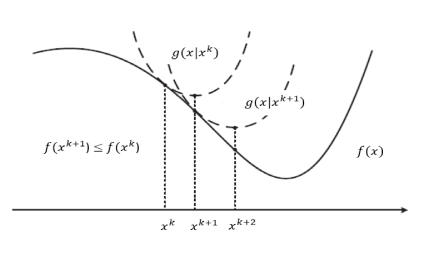
\includegraphics[width=0.5\linewidth]{images/mm-methods.png}
    \caption{\textbf{Intuition for IRLS.} the IRLS scheme majorizes the cost function in the locality of the solution of the previous step by a quadratic function, and then solves for it (note that this general scheme is called majorize-minimize or MM methods). If the quadratic function is chosen appropriately, then each iteration brings closer to the solution. Source:~\cite{noauthor_novel_nodate}.}
    \label{fig:mm-intuition}
\end{figure}

This framework is a powerful tool to solve many complicated problems, and it serves as a proxy to a very wide range of functions. In~\cite{kummerle_denoising_2018, kummerle_understanding_nodate} the authors considered a particularly difficult problem: the rank minimizaton. And in constrast to the nuclear-norm minimization scheme we seen earlier, they have chosen the log-det function as a surrogate to minimize over. It is easy to see how much more powerful this approach is since contrary to nuclear norm, which is only an approximation of the rank, the log-det is equal to the rank. To illustrate that, let us recall that
\[log(x) = \lim_{p \rightarrow 0} \frac{x^p - 1}{p}.\]
Than take $x = \sigma_i(\mathbf{A})$ for some $\mathbf{A}$, and accordingly
\[log(\sigma_i(\mathbf{A})) = \lim_{p \rightarrow 0} \frac{\sigma_i(\mathbf{A})^p - 1}{p}.\]
Next, we make some simple steps
\[\sum_{i=1}^R log(\sigma_i(\mathbf{A})) = \lim_{p \rightarrow 0} \sum_{i=1}^R \frac{\sigma_i(\mathbf{A})^p - 1}{p} =  \frac{\lim_{p \rightarrow 0} \sum_{i=1}^R \sigma_i(\mathbf{A})^p}{p} - \frac{R}{p},\]
and we know that
\[ \lim_{p \rightarrow 0} \sum_{i=1}^R \sigma_i(\mathbf{A})^p = rank(\mathbf{A}).\]
Finally,
\[\sum_{i=1}^R log(\sigma_i(\mathbf{A})^p) = log(\prod_{i=1}^R \sigma_i(\mathbf{A})^p) = log(det(\mathbf{A})),\]
and
\[\frac{\lim_{p \rightarrow 0} \sum_{i=1}^R \sigma_i(\mathbf{A})^p}{p} - \frac{R}{p} = \frac{\norm{\mathbf{A}}_p^p}{p} - \frac{R}{p},\]
where $\norm{\mathbf{A}}_p^p$ is a Schatten-p norm.

Although a deeper discussion of this new algorithm, named Harmonic-Mean-IRLS or HM-IRLS, would be interesting, due to the limitation of this work we need to refer the reader to the doctoral thesis~\cite{kummerle_understanding_nodate} of Christian Kümmerle, or to the the our github repository holding a reference implementation:
\url{https://github.com/hakkelt/IRLS-for-CS-MRI/blob/master/SimpleMatrixCompletion.ipynb}, as the discussion would require a much longer introduction to mathematical concepts. A important property, nevertheless, worth mentioning here: the authors constructed the HM-IRLS to use some second-order information, and as a result of this propoerty, it converges really fast, admitting superlinear convergence in general and even quadratic convergence locally. On the other hand, it also means more heavy computation as well.

\iffalse
\begin{algorithm}
    \SetKwData{Input}{input}
    \SetKwData{Output}{output}
    \Input{
        $y$: under-sampled data\\
        $\Phi$: sampling operator\\
        $\tilde{r}$: rank estimate of solution\\
        $maxIter$: number of CG iteration steps\\
        $N$: number of iterations
        }
    \BlankLine
    initialize: $d_1, d_2$ = size of image, $ϵ^k = \infty, \mathbf{X}^k = \Phi^* \mathbf{y},
    
    \For{$k = 1 \ldots N$}
        $U, \sigma, V = svd(X^k)$\\
        $U^k, σ, V^k = U[:, 1:\tilde{r}], F.S, F.V[:, 1:\tilde{r}]$\\    
        $ϵ^k = min(\epsilon^k, σ[\tilde{r}+1])$\\
        
        $H^k = [1 / (max(\sigma[i], \epsilon^k) * max(\sigma[j], \epsilon^k))  for i in 1:\tilde{r}, j in 1:\tilde{r}]$\\
        $dH^k = [1 / (max(\sigma[\tilde{r}+1], \epsilon^k) * max(\sigma[j], \epsilon^k))  for j in 1:\tilde{r}]$\\
        $P^k([\gamma_1, \gamm_2, \gamm_3]) = U^k * \gamma_1 * V^{k*} + U^k * \gamma_2^T * (I - V^k V^{k*}) + (I - U^k U^k') * \gamma_3^T * V^{k*}$\\
        $^{k*} = [vec(U^{k*} \Phi^* y V^k), U^{k*} * Φᵃy * (I - Vᵏ*Vᵏ')$
                    γ₁ = 
                    γ₂ = 
                    γ₃ = (I - Uᵏ*Uᵏ') * Φᵃy * Vᵏ
                    vcat(, vec(γ₂), vec(γ₃))
                end)
        b = Pᵏ' * Φ' * y
        ��⁻¹ = I / Diagonal(vcat(vec(Hᵏᵤᵥ), vec(kron(dHᵏ, ones(1, d₂))), vec(kron(dHᵏ, ones(1, d₁))')))
        CG_op = FunctionOperator{dType}(name = "CG_op", inDims = (r̃*(r̃+d₁+d₂),), outDims = (r̃*(r̃+d₁+d₂),),
            forw = γ ->  begin
                    (ϵᵏ^2 * I / (��⁻¹ - ϵᵏ^2 * I)) * γ + Pᵏ' * Φ' * Φ * Pᵏ * γ
                end)
        γᵏ = cg(CG_op, b, maxiter = maxIter) # 2.167
        rᵏ = y - Φ * Pᵏ * γᵏ
        γᵏ_tilde = (��⁻¹ / (��⁻¹ - ϵᵏ^2 * I)) * γᵏ - Pᵏ' * Φ' * rᵏ
        Xᵏ = Φ' * rᵏ + Pᵏ * γᵏ_tilde   # 2.168
    end
    
    r, n, s, e = sum(svdvals(Xᵏ) .> 1e-3), opnorm(Xᴳᵀ - Xᵏ, 2), σ[1], ϵᵏ
    n, s, e = @sprintf("%.3f", n), @sprintf("%.3f", s), @sprintf("%.3f", e)
    verbose && println("k = $N,\trank(Xᵏ) = $r,\t‖Xᴳᵀ - Xᵏ‖₂ = $n, σ₁ = $s, ϵᵏ = $e")
    
    Xᵏ
end
\end{algorithm}
\fi

\clearpage % You need \clearpage at the end of every chapter to force images included in this chapter to be rendered in somewhere else